\begin{figure}[H]
\centering
\begin{tikzpicture}[x=1mm,y=1mm,
  input/.style={text width=34mm,minimum height=18mm,inner sep=2.2mm,align=left,
    draw=black!17,fill=black!2,line width=.5pt,font=\small},
  decision/.style={input,text width=49mm,draw=ucasblue!34,fill=ucasblue!7},
  output/.style={input,text width=42mm,draw=agentteal!36,fill=agentteal!5},
  link/.style={-{Latex[length=1.7mm]},draw=ucasblue!63,line width=.58pt},
  head/.style={font=\small\bfseries,text=reportmuted}]
  \node[head] at (0,0) {用户这轮要什么};
  \node[head] at (49,0) {Pi 看了什么、决定什么};
  \node[head] at (102,0) {工具算出或保留什么};
  \node[input] (u1) at (0,-16) {\textbf{1\enspace 截至 18 日初报}\\从可用像元提取候选};
  \node[decision] (d1) at (49,-16) {同轨 7、双极化、共同有效率 100\%\\\textbf{选择 SAR 变化法}};
  \node[output] (p1) at (102,-16) {在线下载、分割并发布\\\textbf{71.19 \km 雷达候选}};
  \node[input] (u2) at (0,-48) {\textbf{2\enspace 更新至 19 日}\\新观测与旧图对照};
  \node[decision] (d2) at (49,-48) {光学共同有效率 96.45\%\\\textbf{改用 MNDWI，引用两期掩膜}};
  \node[output] (p2) at (102,-48) {保留雷达图；新增光学图和四类证据对照};
  \node[input] (u3) at (0,-80) {\textbf{3\enspace 发布核查清单}\\分别算全窗与北部};
  \node[decision] (d3) at (49,-80) {同一套观测、只改变范围\\\textbf{复用对照 ID，调用两次叠加}};
  \node[output] (p3) at (102,-80) {两套独立地图、耕地和路段清单；\textbf{未重下或重分割}};
  \foreach \i in {1,2,3}{
    \draw[link] (u\i.east) -- (d\i.west);
    \draw[link] (d\i.east) -- (p\i.west);
  }
  \draw[link,dashed,draw=agentteal] (p1.south) -- ++(0,-6.3)
    -- node[above,font=\scriptsize,text=agentteal,inner sep=1pt]{复用雷达掩膜} ++(-53,0) -- (d2.north);
  \draw[link,dashed,draw=agentteal] (p2.south) -- ++(0,-6.3)
    -- node[above,font=\scriptsize,text=agentteal,inner sep=1pt]{复用证据对照} ++(-53,0) -- (d3.north);
\end{tikzpicture}
\caption{从三轮真实工具日志整理的决策图。实线是本轮请求和产出，绿色虚线是跨轮复用。第二轮更换观测与算法；第三轮仅改变分析范围。两类判断分别落到不同的工具参数，而不是改变回复措辞。}
\label{fig:karla-decisions}
\end{figure}

\begin{figure}[htbp]
\centering
\begin{tabular}{@{}p{.476\linewidth}@{\hspace{.04\linewidth}}p{.476\linewidth}@{}}
\sffamily\small\bfseries a\enspace 更新观测与证据对照 &
\sffamily\small\bfseries b\enspace 复用证据开展分区核查\\[3pt]
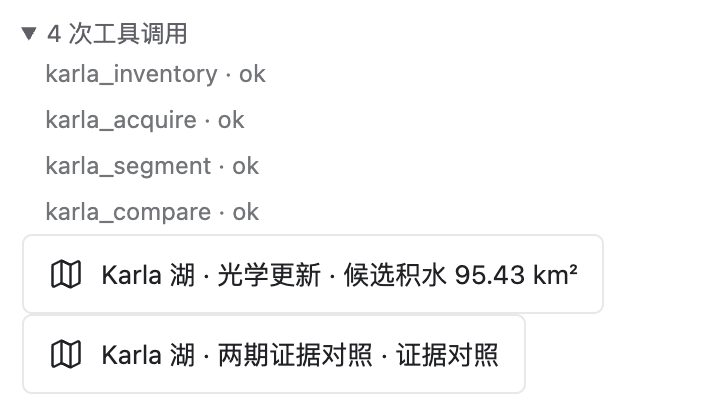
\includegraphics[width=\linewidth]{figures/karla-optical-update.png} &

\includegraphics[width=\linewidth]{figures/karla-reuse-exposure.png}
\end{tabular}
\caption{FloodLab 工作台中的真实执行截图，裁切自同一会话的第二、三轮回复，未改动内容。a：下载、分割和对照均有成功记录，下方是光学更新图与两期对照图；b：只有读取已有资料及两次分区核查的记录，各自对应一个成果入口。}
\label{fig:karla-workbench-traces}
\end{figure}
